
\mode<presentation>
{
  \usetheme{CambridgeUS}
  \usecolortheme{whale}
  \usecolortheme{lily}

  \setbeamercovered{transparent}
  \usefonttheme[onlymath]{serif}
}

\title[\GainandPhaseMarginShortName] % (optional, use only with long paper titles)
{\course: \GainandPhaseMarginName\license}

\subtitle
{Lecture \GainandPhaseMarginNumber} % (optional)


% Delete this, if you do not want the table of contents to pop up at
% the beginning of each subsection:
%\AtBeginSection[]
%{
%  \begin{frame}<beamer>{Outline}
%    \tableofcontents[currentsection,currentsubsection]
%  \end{frame}
%}


% If you wish to uncover everything in a step-wise fashion, uncomment
% the following command:

%\beamerdefaultoverlayspecification{<+->}


\begin{document}

\begin{frame}
  \titlepage
\end{frame}

\mode<article>{
\maketitle
\tableofcontents
}

%\mode<presentation>{
%\begin{frame}{Outline}
%  \tableofcontents
%  % You might wish to add the option [pausesections]
%\end{frame}}
\section{Stability Margins}

If we have a known plant with transfer function $G(s)$, we know how to check to see if a controller $C(s)$ will result in a stable closed loop system

\begin{frame}
\begin{center}
\begin{tikzpicture}[inner sep=0pt,outer sep=0pt,very thick,
sysblock/.style={draw,rectangle,inner sep=2pt,minimum width=1.5cm,minimum height=1.25cm,very thick}]
\draw (-1,0) node[draw,circle] (sum) {$\rule{0pt}{18pt}$};
\draw (1,0) node[sysblock] (G1) {$\plant(s)$};
\draw (1,-2) node[sysblock] (G2) {$H(s)$};
\draw (-2.5,0) node[above=4pt] {$\inptLT(s)$} -- (sum.180) node[above left=4pt] {$+$};
\draw[->] (sum.0) -- node[pos=.5,above=4pt] {$E(s)$} (G1.180);
\draw[->] (G1.0) -- ++(1,0) |- (G2.0);
\draw[->] (G2.180) -| (sum.-90) node[below right] {$-$};
\draw[->] (G1.0) -- ++(2,0) node[above=4pt] {$\outptLT(s)$};
\draw (1,-3.5) node {$\begin{aligned}\outptLT(s)&=\plant(s)E(s)\\E(s) &= \inptLT(s) - H(s)\outptLT(s)\end{aligned}$};


\end{tikzpicture}

\end{center}
\end{frame}

However, what if the plant $G(s)$ is uncertain? For example, the frequency response of $G(s)$ may have been determined from an experiment. Suppose a series of sinusoids of different frequencies were applied to $G(s)$, and we recorded the magnitude and phase shift of the output. The possible results of such an experiment are shown below in blue stars, with the green line indicating a plausible model for the resulting data. One issue with such an experiment is the loss of signal as the output magnitude decreases at high frequency. Usually a sensor has noise characteristics that are constant or perhaps increasing with higher frequency. If the signal we are measuring has lower magnitude at higher frequency, the signal to noise ratio decreases, and our estimates of the magnitude and phase are correspondingly poor. 

\begin{frame}
\begin{center}
\includegraphics[height=3in]{figures/marginsexample1_1}
\end{center}
\end{frame}

Although the green line gives a plausible nominal model, a more conservative approach would be to give upper and lower bounds on the possible magnitude and phase 

\begin{frame}
\begin{center}
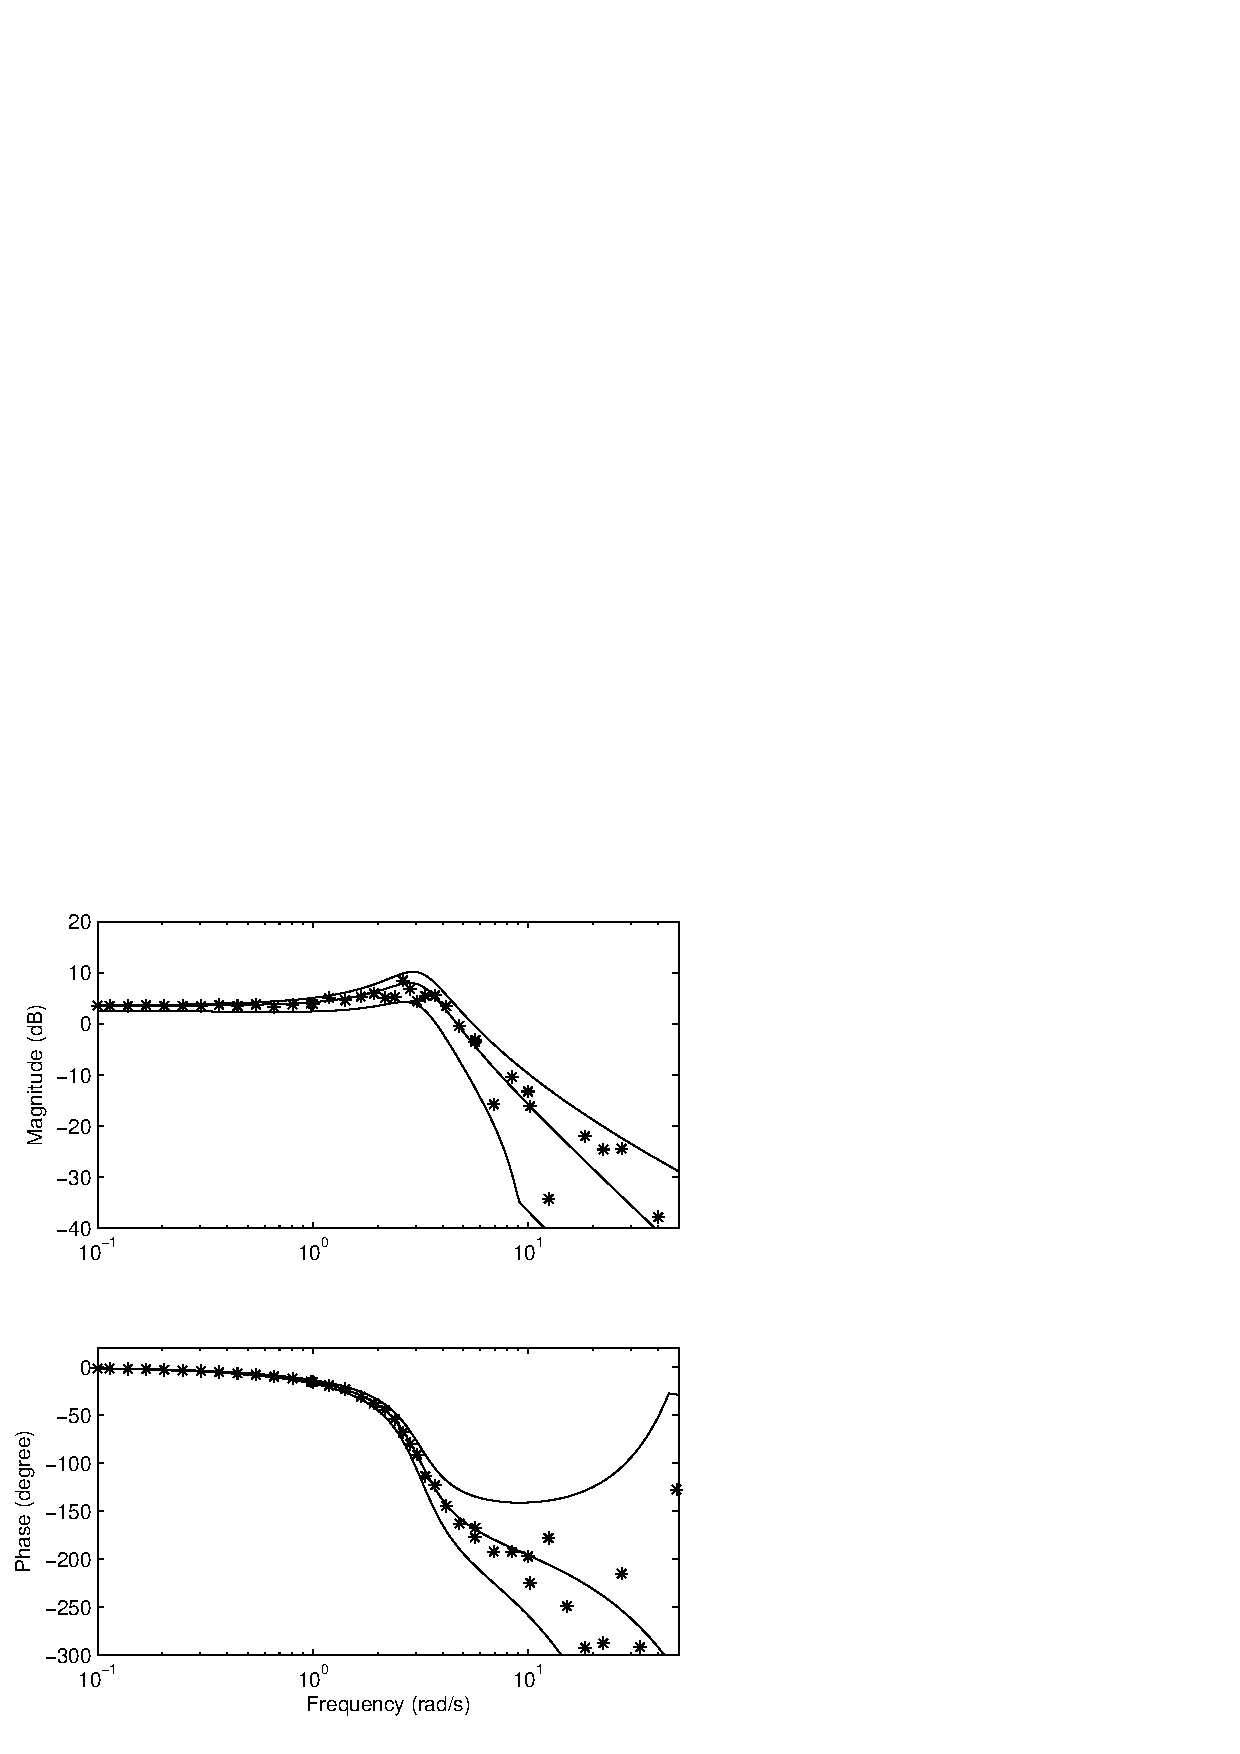
\includegraphics[height=3in]{figures/marginsexample1_2}
\end{center}
\end{frame}
 
Using the nominal model for $G(s)$ and taking $C(s)=1$, the nominal Nyquist plot (shown in blue below) would indicate that the closed loop system is stable. However, if we use the worst case max and min phase and gain, shown by the cyan and red lines, an encirclement of $-1$ cannot be ruled out. In other words, we cannot guarantee closed-loop stability with this $C(s)$ due to the uncertainty in $G(s)$.
\begin{frame}
\begin{center}
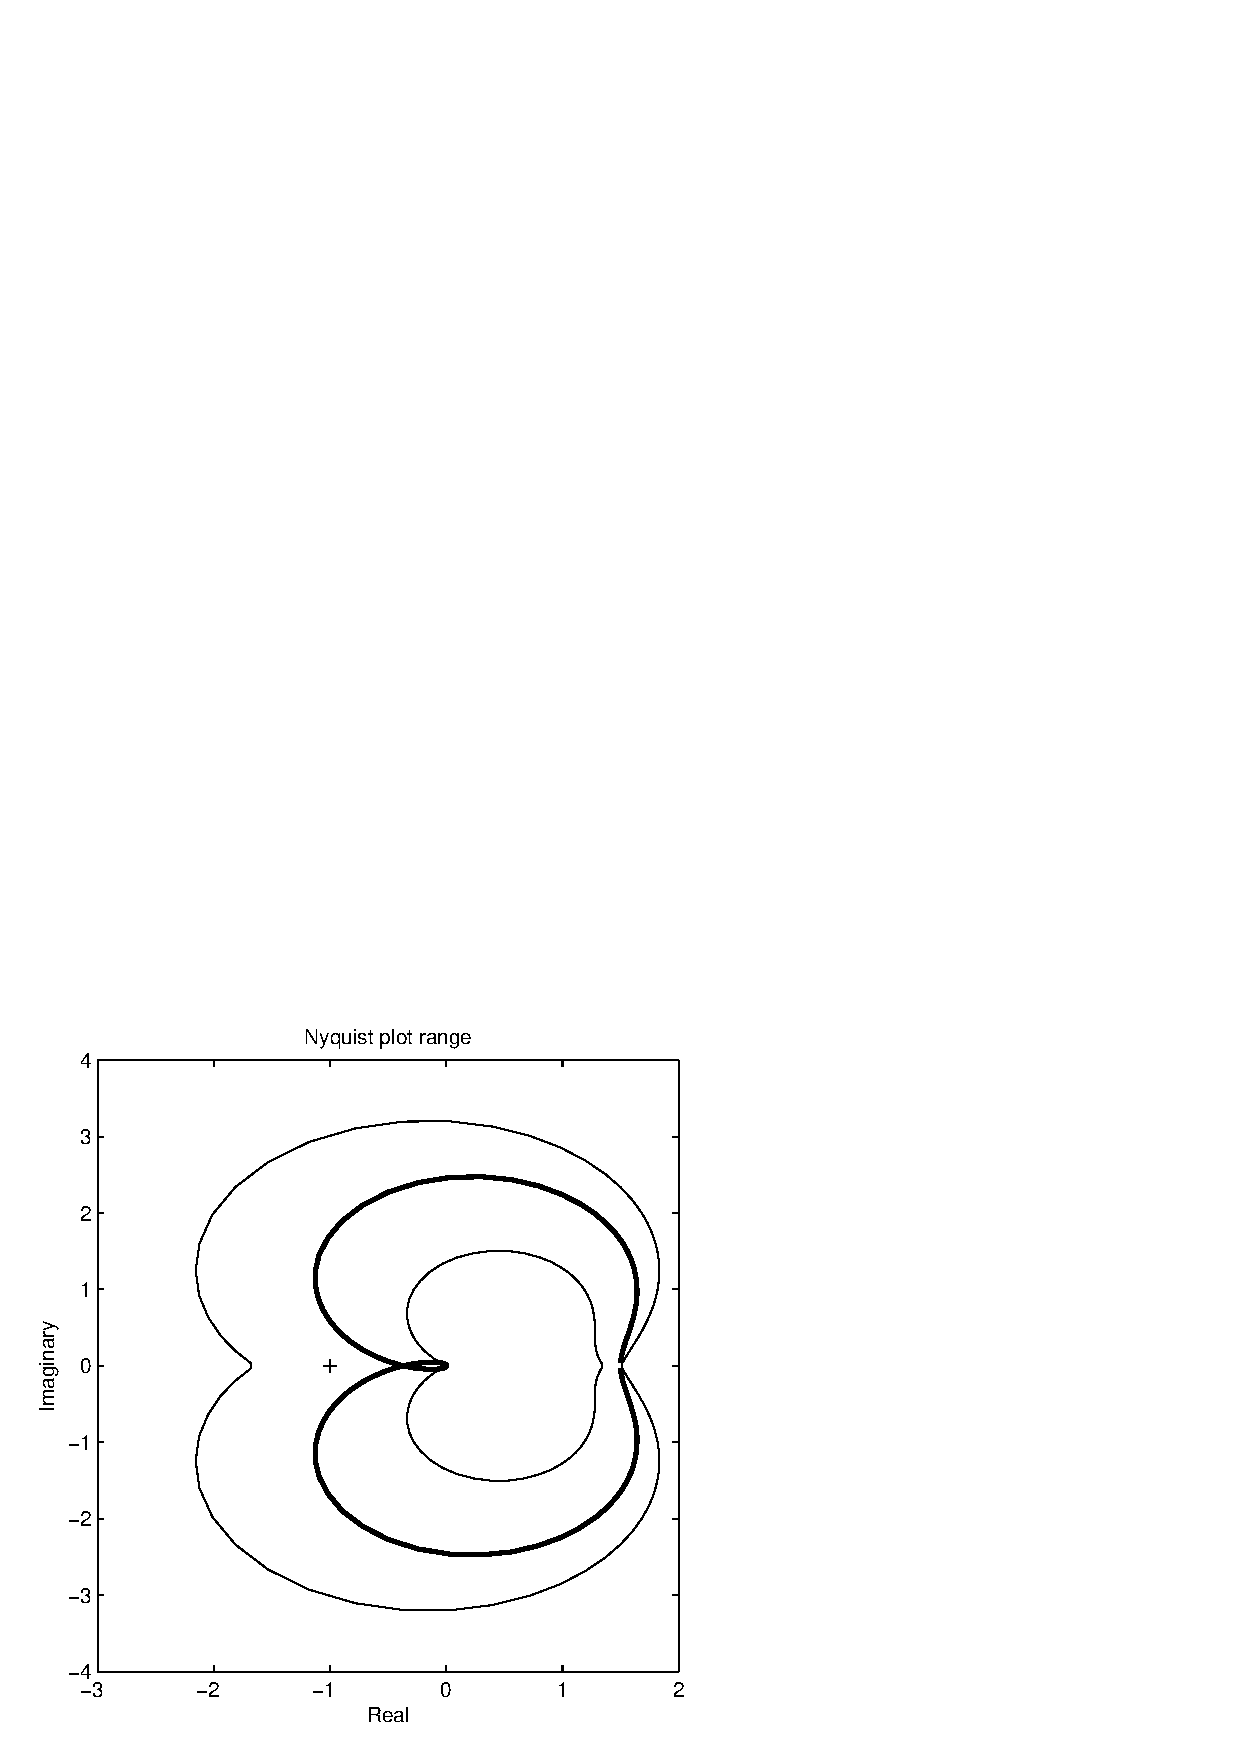
\includegraphics[height=3in]{figures/marginsexample1_4}
\end{center}
\end{frame}

Whether due to uncertainty, changes in dynamics due to system wear and tear, or other effects, a control system needs to be stable not just for the nominal design model, but robust to variations. With the Nyquist stability criterion, if the nominal loop gain is designed to be stable, then the distance of the loop gain to the point $-1+j0$ is a measure of robustness, since if the Nyquist plot crosses $-1+j0$, the number of encirclements must change, and thus the system must go from stability to instability. There are two typical measurements of this distance: the gain margin and the phase margin.

\begin{definition} A {\em gain margin} is a real multiplicative factor $\GM$ such that the Nyquist plot of $\GM L(s)$ will  cross $-1+j0$.
\end{definition}

\begin{definition} The {\em phase margin} is the phase lag $\PM$ such that the Nyquist plot of $e^{-j\PM}L(s)$ will cross $-1+j0$.  
\end{definition}
\section{Gain Margin}

To find the gain margin, we start by searching for the point on the Nyquist plot that will be the one that crosses $-1+j0$ when the loop gain is scaled. A clue is given by the fact that multiplying $L(s)$ by a real number $\GM$ does not change the phase. Since $-1+j0$ has a phase of $-180^{\circ}$ the point that crosses $-1+j0$ must already be on the negative real axis, with a phase of $-180^{\circ}$. This point can be located using either the Bode plot of $L(s)$, or the Nyquist plot. Using the Bode plot, we follow the following steps:

\begin{itemize}
\item Locate where the Bode plot crosses the $-180^{\circ}$ phase line (including any shifts by a multiple of $360^{\circ}$).
\item At those frequencies, go up to the magnitude plot, and determine the distance of the magnitude plot to the $0$~dB line. If the magnitude Bode plot is below $0$ dB, the distance is positive, otherwise the distance is negative. Call this distance $\GMdB$.
\item The gain margin is $\GMdB$ dB, or $\GM = 10^{\GMdB/20}$.
\item If the Bode plot crosses $-180^{\circ}$ multiple times, the smallest margin is taken as the gain margin.
\end{itemize}

\begin{frame}
\mode<article>{\begin{center}}
\hspace{-.24in}
\begin{minipage}{4.7in}
\begin{tikzpicture}
\draw (-6.4,0) node {\includegraphics[height=2.75in]{figures/marginsexample1_5}};
\visible<2->{\draw[thick,red] (-8.55,-1.85) node[left=-3pt] {\tiny$-180$} -- ++(4.5,0); 
\draw[->,dashed,red] (-5.44,-1.85) -- ++(0,3.65);
\draw (-5.37,1.98) node {$\left.\rule{20pt}{0pt}\right\}9$\textsf{dB}};
\draw[thick,red] (-8.55,2.18) -- ++(4.5,0);} 
\draw (0,-.13) node {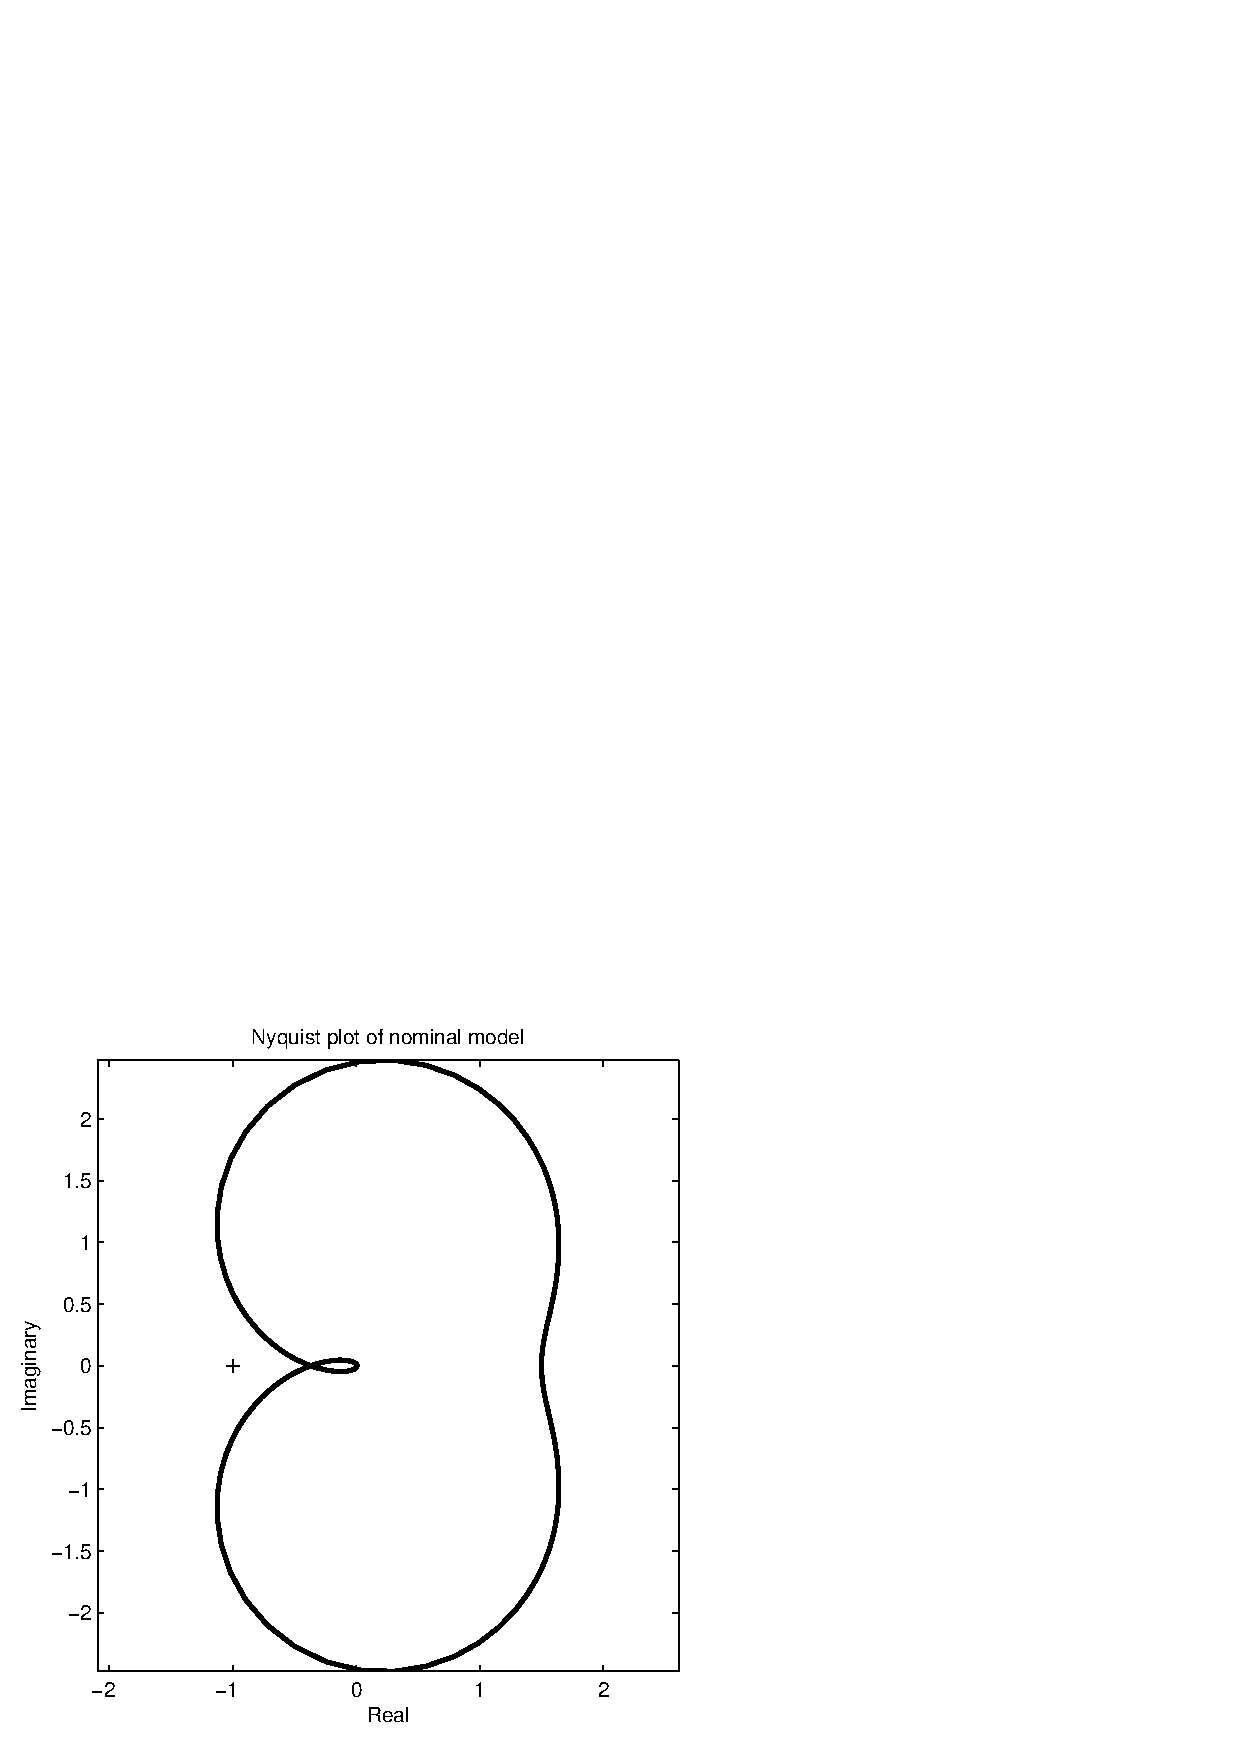
\includegraphics[width=3in]{figures/marginsexample1_3}};
\visible<3->{\draw[thick] (-.65,-.25) -- ++(0,.5);
\draw[->,thick] (-.65,0) -- ++(-.8,0); 
\draw (-.6,-.6) node[right] (a) {$10^{-9/20} = .35$};
\draw (-.6,-1.1) node[right]  {$\GM=10^{9/20} = 2.81$};
\draw[->] (a.180) .. controls ++(180:.25) and ++(-90:.25) .. (-.65,-.25);}
\end{tikzpicture}
\end{minipage}
\mode<article>{\end{center}}
\end{frame}


\section{Phase Margin}

To find the phase margin, again we search for the point on the Nyquist plot that will be the one that crosses $-1+j0$, but this time when the phase is changed. Since only the phase is changed, and $-1+j0$ has a magnitude of $1$, the point we are looking for also has a magnitude of $1$. This point can be found using the following procedure.

\begin{itemize}
\item Locate where the Bode plot crosses the $0$dB magnitude line.
\item At those frequencies, go down to the phase plot, and determine the distance of the phase plot to the $-180^{\circ}$ line. If the phase Bode plot is above $-180^{\circ}$ the distance is positive, otherwise the distance is negative. This is the phase margin $\PM$.
\item If the Bode plot crosses $0$dB multiple times, the smallest margin is taken as the phase margin.
\end{itemize}

\begin{frame}
\mode<article>{\begin{center}}
\hspace{-.24in}
\begin{minipage}{4.7in}
\begin{tikzpicture}
\draw (-6.4,0) node {\includegraphics[height=2.75in]{figures/marginsexample1_5}};
\visible<1->{\draw[thick,red] (-8.55,-1.85) node[left=-3pt] {\tiny$-180$} -- ++(4.5,0); 
\draw[->,dashed,red] (-5.77,2.19) -- ++(0,-3.83);
\draw (-5.96,-1.72) node[right] {\scriptsize$\left.\rule{0pt}{0pt}\right\}25^{\circ}=\PM$};
\draw[thick,red] (-8.55,2.18) -- ++(4.5,0);}
\draw (0,-.13) node {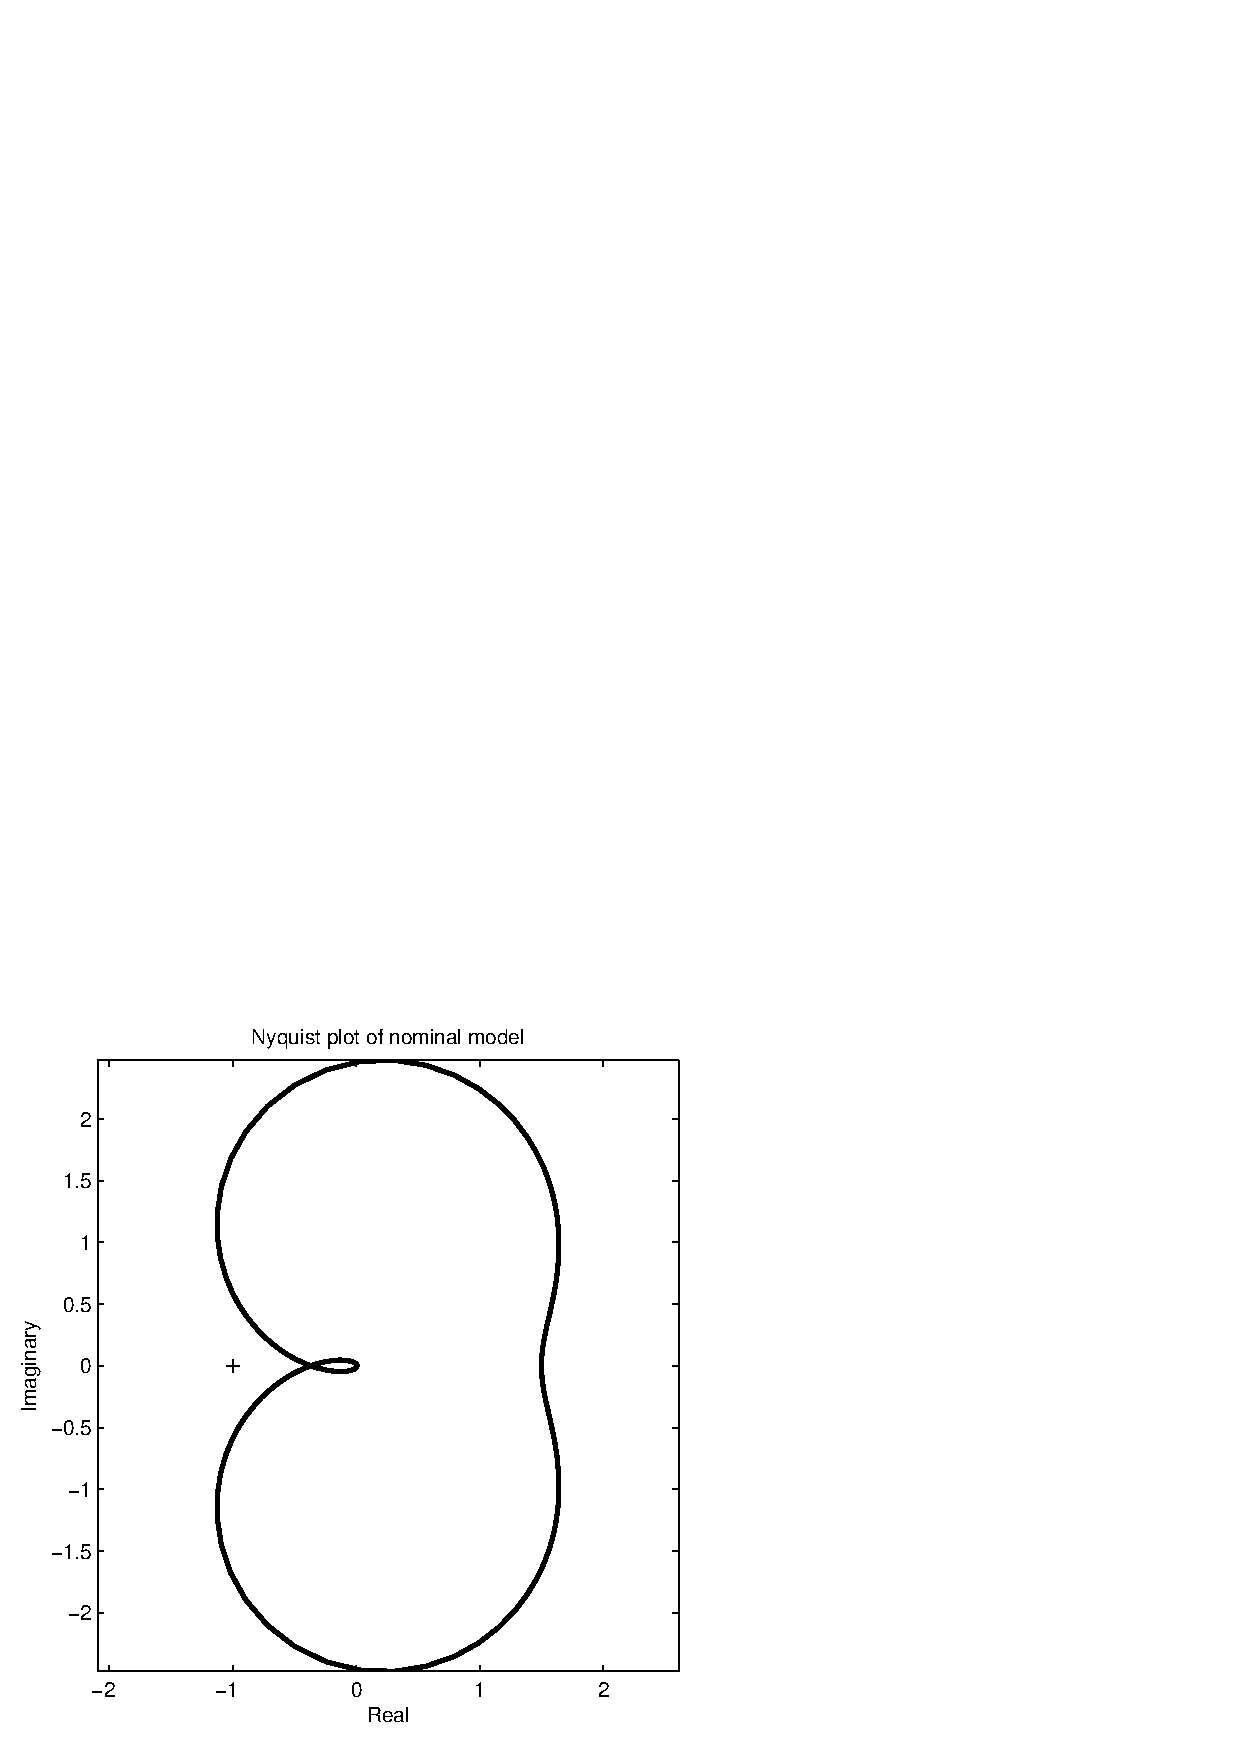
\includegraphics[width=3in]{figures/marginsexample1_3}};
\visible<2->{\draw[-,thick] (-.15,0) -- ++(-155:2); 
\draw[-,dotted] (-.15,0) -- ++(-180:2); 
\draw[dotted] (-.15,0) circle (1.295);
\draw (-.6,0) arc (-180:-155:.45);
\draw (-1.19,-.18) node {$\PM$};}
\end{tikzpicture}
\end{minipage}
\mode<article>{\end{center}}
\end{frame}

\section{Example}

\begin{example}
Determine the stability margins for the following feedback system

\begin{frame}
\begin{center}
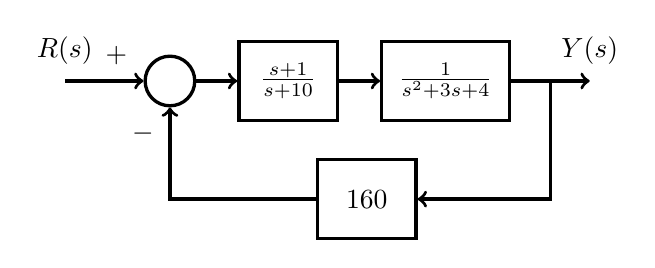
\begin{tikzpicture}[very thick,
sysblock/.style={draw,rectangle,inner sep=6pt,minimum width=1.25cm,minimum height=1.0cm,very thick},
summer/.style={circle,draw,very thick}]

\draw (0,0) node[summer] (sum) {\rule{10pt}{0pt}};
\draw (1.5,0) node[sysblock] (C) {$\frac{s+1}{s+10}$};


\draw (3.5,0) node[sysblock] (G) {$\frac{1}{s^2+3s+4}$};

\draw (2.5,-1.5) node[sysblock] (H) {$160$};

\draw[<-] (sum.180) node[above left=2pt] {$+$} -- ++(-1,0) node[above=2pt] {$R(s)$};
\draw[->] (sum.0) -- (C.180);
\draw[->] (C.0) -- (G.180);
\draw[->] (G.0) -- ++(0.5,0) |- (H.0);
\draw[->] (H.180)  -| (sum.-90) node[below left=2pt] {$-$};
\draw[->] (G.0) ++(0.5,0) -- ++(0.5,0) node[above=2pt] {$Y(s)$};

\end{tikzpicture}
\end{center}
\end{frame}

The Bode plot and Nyquist plot for this system are shown below

\begin{frame}
\begin{center}
\mode<article>{\includegraphics[height=2.3in]{figures/example1_1}
\includegraphics[height=2.3in]{figures/example1_2}}
\mode<presentation>{\includegraphics[height=2.3in]{figures/example1_1}
\raisebox{.65in}{\includegraphics[height=1in]{figures/example1_2}}}
\end{center}
\end{frame}

\begin{itemize}
\item Gain Margin:
\begin{itemize}
\item Where is the phase $-180^{\circ}$? Answer: 0.8 rad/s
\item What is the magnitude at 0.8 rad/s? Answer: -6 dB
\item Gain margin: 6 dB or $10^{6/20}=2$
\end{itemize}
\item Phase Margin:
\begin{itemize}
\item Where is the magnitude 0 dB? Answer 0.6 rad/s
\item What is the phase at 0.6 rad/s? $-157^{\circ}$
\item Phase margin: 180-157=23$^{\circ}$
\end{itemize}
\end{itemize}
\end{example}\qed

Sometimes the gain or phase margin can be infinite, if there is no shift that can make the system unstable, as shown in the next example.

\begin{example}
Determine the stability margins for the following feedback system

\begin{frame}
\begin{center}
\input{figures/example2blockdiagram.tex}
\end{center}
\end{frame}

The Bode plot and Nyquist plot for this system are shown below

\begin{frame}
\begin{center}
\mode<article>{\includegraphics[height=2.3in]{figures/example2_1}
\includegraphics[height=2.3in]{figures/example2_2}}
\mode<presentation>{\includegraphics[height=2.3in]{figures/example2_1}
\raisebox{.65in}{\includegraphics[height=1.0in]{figures/example2_2}}}
\end{center}
\end{frame}

Note that Matlab does not add the effect of the notch due to a pole at $s=0$, thus we must mentally complete the Nyquist plot by adding a semi-circle on the right.

\begin{itemize}
\item Gain Margin:
\begin{itemize}
\item Where is the phase $-180^{\circ}$? Answer: No finite frequency!
\item Since the phase does not reach $-180^{\circ}$ until $\omega=\infty$ (and the magnitude decreases at high frequency) a shift in gain cannot destabilize the system
\item Gain margin: infinite.
\end{itemize}
\item Phase Margin:
\begin{itemize}
\item Where is the magnitude 0 dB? Answer 0.8 rad/s
\item What is the phase at 0.8 rad/s? $-128^{\circ}$
\item Phase margin: 180-128=52$^{\circ}$
\end{itemize}
\end{itemize}


\end{example}\qed

\section{Lecture Highlights}
The primary takeaways from this article include
\begin{enumerate}
\setlength{\itemsep}{5pt}
\setlength{\parskip}{0pt}
\setlength{\parsep}{0pt}
\item Gain and phase margins are measures of robustness of a system to uncertainty; in other words, how far can the model be ``off'' before we are in danger the closed-loop system becoming unstable?
%\item The gain margin (GM) is found on the magnitude Bode plot at the frequency where the phase Bode plot crosses $-180^\circ$. The phase margin (PM, or $\phi_{PM}$) is found on the phase Bode plot at the crossover frequency $\omega_{co}$ where the magnitude Bode plot crosses 0 dB.
\item The gain and phase margins can be found from the Bode plot or the Nyquist plot. When comparing the two, remember to use the dB log conversions.
\item Both gain and phase margins can be infinity, which is a strong result for stability considerations.
\end{enumerate}


\section{Quiz Yourself}

\subsection{Questions}

\begin{enumerate}
\setlength{\itemsep}{5pt}
\setlength{\parskip}{0pt}
\setlength{\parsep}{0pt}
\item Consider a unity gain feedback system
\begin{center}
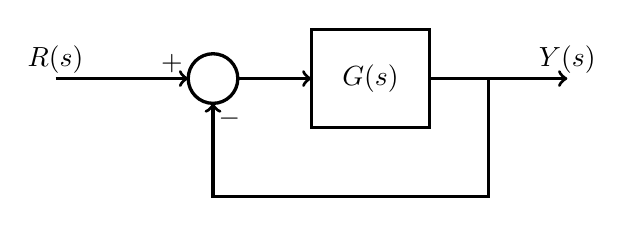
\begin{tikzpicture}[scale=1,inner sep=0pt,outer sep=0pt,very thick,
sysblock/.style={draw,rectangle,inner sep=2pt,minimum width=1.5cm,minimum height=1.25cm,very thick}]
\draw (2,0) node[draw,circle] (sum1) {$\rule{0pt}{18pt}$};
\draw (4,0) node[sysblock] (Kp) {$G(s)$};
\draw[->] (0,0) node[above=2pt] {$R(s)$} -- (sum1.180) node[above left=2pt] {$+$};
\draw[->] (sum1.0) --  (Kp);
\draw[->] (Kp) -- ++(2.5,0) node[above=2pt] {$Y(s)$};
\draw[->] (Kp) ++(1.5,0) -- ++(0,-1.5) -| (sum1.-90) node[below right=2pt] {$-$};
\end{tikzpicture}
\end{center}
If $G(s)$ is stable and has the following Bode plot, determine if the system is closed loop stable, and if so, find the phase and gain margin.
\begin{center}
\includegraphics[width=5.5in]{quizfigures/prob1}
\end{center}
\end{enumerate}


\subsection{Solutions}
\begin{enumerate}
\setlength{\itemsep}{5pt}
\setlength{\parskip}{0pt}
\setlength{\parsep}{0pt}
\item \rule{12pt}{0pt}
\begin{center}
\includegraphics[width=6in]{quizfigures/1asoln}\\
\includegraphics[width=6in]{quizfigures/1bsoln}\\
\includegraphics[width=6in]{quizfigures/1csoln}
\end{center}
\end{enumerate}



\end{document}


